\documentclass{article}
\usepackage{graphicx} % Required for inserting images
\usepackage{xcolor}
\usepackage{float}
\usepackage{tikz}
\usetikzlibrary{patterns}
\usepackage{array}

% --- STATE message figure (Description of Messages): colours and helper macros ---
\definecolor{msgfill}{HTML}{F2F3F5}\definecolor{msgdraw}{HTML}{9AA1AD}
\definecolor{stampc}{HTML}{1F3F75}
\definecolor{setfill}{HTML}{FFFFFF}\definecolor{setdraw}{HTML}{8C929C}
\definecolor{actfill}{HTML}{FFFFFF}\definecolor{actdraw}{HTML}{8C929C}
\definecolor{statefill}{HTML}{FFFFFF}\definecolor{statedraw}{HTML}{B4BCC8}
\definecolor{delfill}{HTML}{F8CECC}\definecolor{deldraw}{HTML}{B85450}
% single-line field: [extra style] {x}{y}{width}{text}
\newcommand{\lofisfld}[5][]{\node[draw=black!55, fill=white, rounded corners=1pt, minimum width=#4cm, minimum height=0.5cm, inner sep=2pt, font=\footnotesize, #1] at (#2,#3) {#5};}
% stamp <version, node ID>
\newcommand{\lofistamp}[2]{\textcolor{stampc}{$\langle$#1, #2$\rangle$}}
% field box: [extra style] {x}{y}{width}{value}{stamp}
\newcommand{\lofifld}[6][]{\node[draw=black!55, fill=white, rounded corners=1pt, minimum width=#4cm, minimum height=0.62cm, inner sep=1pt, align=center, font=\footnotesize, #1] at (#2,#3) {#5\\[-2pt]{\scriptsize\color{black!60}#6}};}
% step cell: {index 0-7}{y}{on|off}{stamp}
\newcommand{\loficell}[4]{\pgfmathsetmacro\cx{4.2+#1*0.88+floor(#1/4)*0.14+0.41}\node[#3, minimum width=0.82cm, minimum height=0.62cm, inner sep=0, rounded corners=1pt, align=center, font=\scriptsize] at (\cx,#2) {#3\\[-2pt]{\color{.!75}#4}};}

% let tall figures sit at the top of a page with text below, instead of on a page of their own
\renewcommand{\topfraction}{0.85}
\renewcommand{\textfraction}{0.1}
\renewcommand{\floatpagefraction}{0.75}

\setlength{\parindent}{0pt}
\setlength{\parskip}{4pt}

\title{Distributed Systems Design Plan (Group 10) - \\
    Lö-Fi: Real-Time Multiplayer Drum Sequencer}
\author{Sami Heinimo, Boris Banchev, Akseli Kokki,\\
    Katri Laamala, Jasse Merivirta}
\date{November 2026}

\begin{document}

\maketitle

\newpage
\tableofcontents
\newpage

\section{General Description}

With Lö-Fi, musicians and hobbyists alike can collaborate and create music together. The final product will be a drum sample sequencer, where users can edit the sequence in real time. In practice, the sequence will consist of individual tracks, each of which can be modified at any time. A track $A$ at time $x$ can be either in an on or off state, signifying whether the sample saved to track $A$ is played at that point in time. The changes made should be visible to other users immediately, and the global state should change along with any modifications on all nodes.

The viewpoints required by the course are covered as follows:

\begin{itemize}
    \setlength{\itemsep}{0pt}
    \item \textbf{Global state:} every node holds a copy of the sequencer state (Global state and consistency).
    \item \textbf{Consistency and synchronization:} every value in the state has a version stamp, and all nodes merge incoming copies with the same rule. Playback follows a shared clock (Global state and consistency, Playhead synchronization).
    \item \textbf{Consensus:} the nodes elect a time reference with the bully algorithm (Playhead synchronization).
    \item \textbf{Fault tolerance:} a failed node is noticed from its missing heartbeats, and the session continues without it (Fault tolerance).
    \item \textbf{Scalability:} sessions are independent of each other, and in a large session each node would connect to only some of the others (Scalability).
\end{itemize}

\section{Architecture and nodes}

Lö-Fi is based on a peer-to-peer architecture with two kinds of nodes: \textbf{peer} nodes and \textbf{bootstrap} nodes (Figure~\ref{fig:node_architecture}).

A peer node is an instance of the application running on a user's computer with its own IP address. There is no separate client or server: the same process runs the sequencer interface, stores a local copy of the session's global state and handles all communication with other nodes. The peer nodes run on separate virtual machines. Each node generates a unique node ID when it starts, which identifies the sender of every update and is used to break ties between conflicting updates.

Bootstrap nodes are always-online servers whose addresses are hardcoded into the application. Their only role is to be the first point of contact for new peers in the control plane. They never join a session cluster and never hold sequencer state.

\begin{figure}[H]
    \centering
    \includegraphics[width=0.9\linewidth]{graphics/lofi_node_architecture.png}
    \caption{Node architecture for Lö-Fi: the top half contains the control plane, where nodes find others based on a magnet link. The lower half contains the data plane, where session clusters are formed and nodes are connected to each other.}
    \label{fig:node_architecture}
\end{figure}

\subsection{Joining and leaving a session}

Nodes will connect to each other with a mechanism based on BitTorrent; initial connections will be made using bootstrap nodes. The connecting node pings a bootstrap node, which introduces it to a few active peers.

The connecting node either hosts a new session or joins an existing one. Sessions are managed via a global distributed hash table (DHT), which is stored across the peer nodes themselves. If the connecting node hosts a new session, the session ID is added to the DHT as a key, with the host's IP address as the corresponding value. If the node joins an existing session, it queries the DHT for a session ID (obtained via magnet link), and gets the IPs of peers in the session as a response. The joining node then sends a JOIN message to one of these peers, which answers with a STATE message. From the members part of that state, the new node learns about the rest of the session and starts sending its own STATE messages.

Once a node is a member of a session, it also stores its own IP address under the session ID in the DHT. This keeps the session reachable after the host has left and is the reason a DHT lookup returns several peers. When a node leaves, it removes its IP address from the session's DHT entry.

Figure~\ref{fig:node_architecture} shows the same peer at both stages: as the Joining User Node in the control plane, and as Node 1 in session cluster A101 after it has joined.

\subsection{Roles within a session}

Once P2P connections are established, the nodes are isolated within their own session clusters. Within the session, each node is connected to every other node, allowing for low-latency data transfer as well as robust redundancy in case of failing nodes.

All peer nodes in a session have the same role. No node is a master and every node can edit the sequence. The host of a session is only special while creating it and is an ordinary peer afterwards. A node can only change its own local copy of the state directly. It affects other nodes by sending them its copy, which each receiver merges into its own with the same rule (see Global state and consistency). Because every node applies this rule identically, the tiebreak on node IDs gives no node extra authority. The only special role is the time reference, which the other nodes get their clock from (see Playhead synchronization). It has no say over the state.

Throughout the session each node logs important events, such as joins, leaves, and sent and received updates. This makes debugging easier and helps to show that the system works correctly.

\section{Global state and consistency}

Every node holds a copy of the session's global state (Figure~\ref{fig:state_message}). The state has four parts: settings such as the tempo and the step count, the playback state, the tracks, and the members.

\begin{figure}[htbp]
\centering
\resizebox{\linewidth}{!}{%
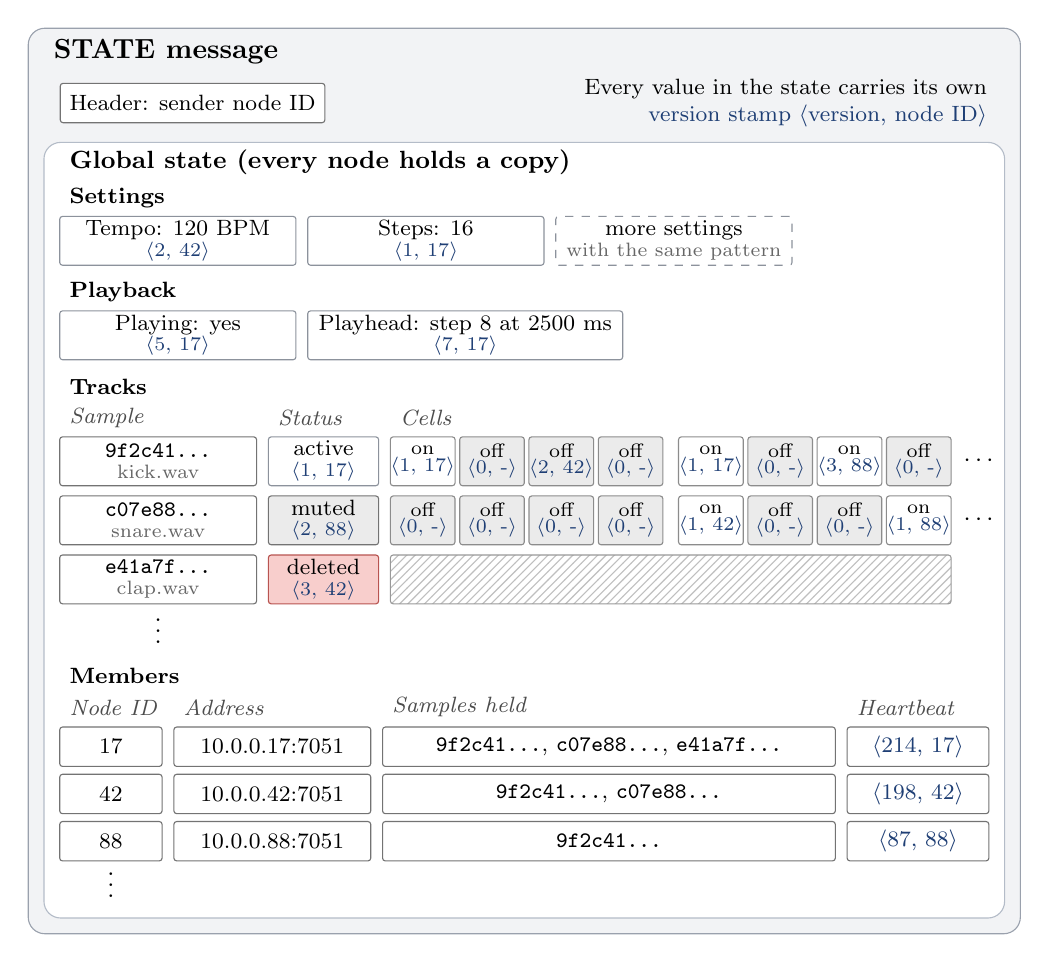
\begin{tikzpicture}[x=1cm, y=1cm, font=\small,
    on/.style={draw=black!45, fill=white},
    off/.style={draw=black!45, fill=black!8},
    hdr/.style={font=\footnotesize\itshape, text=black!70, anchor=west},
    sec/.style={font=\footnotesize\bfseries, anchor=west}]
  % STATE message
  \draw[draw=msgdraw, fill=msgfill, rounded corners=6pt] (-0.4,3.0) rectangle (12.2,-8.5);
  \node[anchor=west, font=\bfseries] at (-0.2,2.7) {STATE message};
  \node[draw=black!55, fill=white, rounded corners=1pt, minimum height=0.5cm, font=\footnotesize, anchor=west] at (0,2.05) {Header: sender node ID};
  \node[align=right, font=\footnotesize, anchor=east] at (11.9,2.05) {Every value in the state carries its own\\\textcolor{stampc}{version stamp $\langle$version, node ID$\rangle$}};
  % global state
  \draw[draw=statedraw, fill=statefill, rounded corners=6pt] (-0.2,1.55) rectangle (12.0,-8.3);
  \node[anchor=west, font=\small\bfseries] at (0,1.3) {Global state (every node holds a copy)};
  % settings
  \node[sec] at (0,0.85) {Settings};
  \lofifld[draw=setdraw, fill=setfill]{1.5}{0.3}{3.0}{Tempo: 120 BPM}{\lofistamp{2}{42}}
  \lofifld[draw=setdraw, fill=setfill]{4.65}{0.3}{3.0}{Steps: 16}{\lofistamp{1}{17}}
  \lofifld[draw=setdraw, dashed]{7.8}{0.3}{3.0}{more settings}{with the same pattern}
  % playback
  \node[sec] at (0,-0.35) {Playback};
  \lofifld[draw=setdraw, fill=setfill]{1.5}{-0.9}{3.0}{Playing: yes}{\lofistamp{5}{17}}
  \lofifld[draw=setdraw, fill=setfill]{5.15}{-0.9}{4.0}{Playhead: step 8 at 2500 ms}{\lofistamp{7}{17}}
  % tracks and members sit one row lower
  \begin{scope}[yshift=-1.2cm]
  % tracks
  \node[sec] at (0,-0.35) {Tracks};
  \node[hdr] at (0,-0.75) {Sample};
  \node[hdr] at (2.65,-0.75) {Status};
  \node[hdr] at (4.2,-0.75) {Cells};
  % track A
  \lofifld{1.25}{-1.3}{2.5}{\texttt{9f2c41\ldots}}{kick.wav}
  \lofifld[draw=actdraw, fill=actfill]{3.35}{-1.3}{1.4}{active}{\lofistamp{1}{17}}
  \loficell{0}{-1.3}{on}{\lofistamp{1}{17}} \loficell{1}{-1.3}{off}{\lofistamp{0}{-}} \loficell{2}{-1.3}{off}{\lofistamp{2}{42}} \loficell{3}{-1.3}{off}{\lofistamp{0}{-}}
  \loficell{4}{-1.3}{on}{\lofistamp{1}{17}} \loficell{5}{-1.3}{off}{\lofistamp{0}{-}} \loficell{6}{-1.3}{on}{\lofistamp{3}{88}} \loficell{7}{-1.3}{off}{\lofistamp{0}{-}}
  \node at (11.67,-1.3) {$\cdots$};
  % track B
  \lofifld{1.25}{-2.05}{2.5}{\texttt{c07e88\ldots}}{snare.wav}
  \lofifld[fill=black!8]{3.35}{-2.05}{1.4}{muted}{\lofistamp{2}{88}}
  \loficell{0}{-2.05}{off}{\lofistamp{0}{-}} \loficell{1}{-2.05}{off}{\lofistamp{0}{-}} \loficell{2}{-2.05}{off}{\lofistamp{0}{-}} \loficell{3}{-2.05}{off}{\lofistamp{0}{-}}
  \loficell{4}{-2.05}{on}{\lofistamp{1}{42}} \loficell{5}{-2.05}{off}{\lofistamp{0}{-}} \loficell{6}{-2.05}{off}{\lofistamp{0}{-}} \loficell{7}{-2.05}{on}{\lofistamp{1}{88}}
  \node at (11.67,-2.05) {$\cdots$};
  % track C (deleted: tombstone)
  \lofifld{1.25}{-2.8}{2.5}{\texttt{e41a7f\ldots}}{clap.wav}
  \lofifld[draw=deldraw, fill=delfill]{3.35}{-2.8}{1.4}{deleted}{\lofistamp{3}{42}}
  \draw[draw=black!40, pattern=north east lines, pattern color=black!25, rounded corners=1pt] (4.2,-3.11) rectangle (11.32,-2.49);
  \node at (1.25,-3.35) {$\vdots$};
  % members
  \node[sec] at (0,-4.025) {Members};
  \node[hdr] at (0,-4.425) {Node ID};
  \node[hdr] at (1.45,-4.425) {Address};
  \node[hdr] at (4.1,-4.425) {Samples held};
  \node[hdr] at (10.0,-4.425) {Heartbeat};
  \lofisfld{0.65}{-4.925}{1.3}{17}
  \lofisfld{2.7}{-4.925}{2.5}{10.0.0.17:7051}
  \lofisfld{6.975}{-4.925}{5.75}{\texttt{9f2c41\ldots}, \texttt{c07e88\ldots}, \texttt{e41a7f\ldots}}
  \lofisfld{10.9}{-4.925}{1.8}{\lofistamp{214}{17}}
  \lofisfld{0.65}{-5.525}{1.3}{42}
  \lofisfld{2.7}{-5.525}{2.5}{10.0.0.42:7051}
  \lofisfld{6.975}{-5.525}{5.75}{\texttt{9f2c41\ldots}, \texttt{c07e88\ldots}}
  \lofisfld{10.9}{-5.525}{1.8}{\lofistamp{198}{42}}
  \lofisfld{0.65}{-6.125}{1.3}{88}
  \lofisfld{2.7}{-6.125}{2.5}{10.0.0.88:7051}
  \lofisfld{6.975}{-6.125}{5.75}{\texttt{9f2c41\ldots}}
  \lofisfld{10.9}{-6.125}{1.8}{\lofistamp{87}{88}}
  \node at (0.65,-6.575) {$\vdots$};
  \end{scope}
\end{tikzpicture}}
\caption{The global state as it is carried in a STATE message. Every value has its own version stamp $\langle$version, node ID$\rangle$.}
\label{fig:state_message}
\end{figure}

The playback state says whether the sequencer is playing and where the playhead is, given as the step it was on at a certain session time (see Playhead synchronization). A node that changes the tempo or presses play or stop also updates this position. A track is identified by the hash of its sample and has a status (active, muted or deleted) and one cell per step, which is either on or off. Deleted tracks stay in the state, so that an older copy of the state cannot bring them back. A member entry contains the node's address and the samples it holds.

Every value in the state has its own version stamp $\langle$version, node ID$\rangle$. When a node changes a value, it increases the version by one and sets the node ID to its own. After every local change, and also at a fixed interval, a node sends a STATE message to all members of the session. The message carries the node's whole state and its node ID. When a node receives a STATE message, it compares each value with its own copy and keeps the one with the higher version; if the versions are equal, the higher node ID wins. In effect, every value has its own Lamport clock, with the node ID as the tiebreak. The result is a last-writer-wins rule applied to each value separately.

All nodes apply the same rule, so they end up with the same state regardless of the order in which messages arrive, and a lost message is covered by the next one. This is why STATE messages can be sent over UDP. The consistency level we aim for is eventual consistency: the copies may differ for a moment, but they converge to the same state.

\section{Playhead synchronization}

All nodes in a session should play the same step at the same moment, so that the music sounds the same on every machine. Sending the playhead position in messages would not achieve this, because every message arrives after a different delay. Instead, the nodes keep a shared clock, which we call session time, and each node computes the playhead position from that clock and the state.

For the shared clock we plan to use the technique behind NTP, which was covered on the course. One node in the session is the time reference. The other nodes regularly ask it for the time and correct the answer for the network delay. The reference is chosen with the bully algorithm, in which the live node with the highest node ID wins. Choosing the reference is a consensus problem, since all nodes have to agree on the same node.

Our goal is to keep the nodes within about 10 ms of each other, possibly also correcting for each machine's individual audio output latency.

\section{File sharing}

Each member can add a new track and a sample file to be played on the track.
The sample file is eventually distributed to all other members.
The sample file size is relatively small, maximum of a few megabytes.
File names are hashed file contents to avoid conflicts with similarly named files.

Distribution of files is a pull-based system.
When a new file is added to the system the other members learn about it from the next STATE message.
Part of the global state is a list of tracks and, for each member, a list of the files it has.
Any node can request a specific file from another node.
This happens if a node notices it's missing a file it should have.
When a node has successfully pulled a sample file from another node it adds the file to its own member entry, so everyone sees from its next STATE message that it also has the file.

The requesting node handles transfer failures.
If a request times out it asks some other node or the same node again.
Data is transferred via a dedicated TCP connection as transfers should not block sequencer messages.
A node can limit its concurrent uploads so it does not block on sequencer messages.

\section{Fault tolerance}

Every node holds the whole state, so a session does not depend on any single node. If a node fails without warning, the remaining nodes continue the session with their own copies of the state.

Failures are detected with heartbeats. Every time a node sends a STATE message, it increases the version of its own member entry, and the periodic STATE messages make sure this happens regularly. If a member's version has not increased for longer than a timeout, the other nodes consider that member gone.

If the time reference fails, a new election picks another node. If the network splits, each part elects its own reference, and the parts line up again once they reconnect.

Since a node needs the bootstrap nodes only for its first contact with the network, a failing bootstrap node does not affect sessions that are already running.

\section{Scalability}

New sessions can be created without affecting existing sessions at all, as the nodes only connect to others within the same session. As a result, the number of sessions is unlimited.

The size of a single session is a more difficult question. With a low number of nodes within a session, every node connecting to every other node is a feasible solution. However, if the number of nodes within the session grows, it becomes less and less sustainable to send every message to every other node. At some cutoff, the within-session architecture will change; instead of connecting to every other node, each node connects to a subset of all the nodes within the session. For example, node 1 will connect to node 2 and node 3, while node 2 connects to nodes 3 and 4. In practice, every node would connect to a larger subset (e.g.\ to 20 other nodes), providing robust fault tolerance while retaining low latency. Changes could then spread through the session as in a gossip-based protocol: a node sends its STATE messages only to its neighbours, whose own STATE messages carry the changes onward. In such a session a node would synchronize its clock through a neighbour, as in NTP's strata.

\section{Messages}

Table~\ref{tab:messages} lists the messages that a peer node sends and receives. Only the STATE message is designed in detail (Figure~\ref{fig:state_message}). The other messages are tentative, and the format of the bootstrap and DHT messages will depend on the DHT implementation we end up using.

\begin{table}[htbp]
\centering
\footnotesize
\renewcommand{\arraystretch}{1.2}
\begin{tabular}{@{}>{\raggedright\arraybackslash}p{2.2cm}>{\raggedright\arraybackslash}p{3.2cm}>{\raggedright\arraybackslash}p{3.2cm}>{\raggedright\arraybackslash}p{2.2cm}@{}}
\hline
\textbf{Message} & \textbf{From, to} & \textbf{When} & \textbf{Notes} \\
\hline
STATE & every node to all members of its session & after every local change and at a fixed interval & whole state, over UDP \\
JOIN & joining node to one member & when joining a session & answered with a STATE message \\
Bootstrap and DHT messages & node to a bootstrap node or the DHT & first contact; hosting, joining or leaving & not designed yet \\
Time request and reply & node to the time reference and back & regularly & not designed yet \\
Election messages & between the members of a session & when a time reference has to be chosen & bully algorithm, not designed yet \\
File request & node to a member that holds the sample & when a sample is missing & file returned over TCP \\
\hline
\end{tabular}
\caption{Messages sent and received by a peer node.}
\label{tab:messages}
\end{table}

\end{document}
